% This is LLNCS.DEM the demonstration file of
% the LaTeX macro package from Springer-Verlag
% for Lecture Notes in Computer Science,
% version 2.4 for LaTeX2e as of 16. April 2010
%
\documentclass{llncs}

% allows for temporary adjustment of side margins
\usepackage{chngpage}

% just makes the table prettier (see \toprule, \bottomrule, etc. commands below)
\usepackage{booktabs}

\usepackage[utf8]{inputenc}

% URL handling
\usepackage{url}
\urlstyle{same}

% footnotes
\usepackage{scrextend}

% Todos
%\usepackage[colorinlistoftodos]{todonotes}
%\newcommand{\ke}[1]{\todo[size=\small, color=orange!40]{\textbf{Kai:} #1}}
%\newcommand{\tb}[1]{\todo[size=\small, color=green!40]{\textbf{Thomas:} #1}}


%\usepackage{makeidx}  % allows for indexgeneration

%\usepackage{amsmath}
\usepackage{amsmath, amssymb}
\usepackage{mathabx}

% monospace within text
\newcommand{\ms}[1]{\texttt{#1}}

%\usepackage{listings}% http://ctan.org/pkg/listings
%\lstset{
  %numbers=left,numbersep=2mm,frame=single,mathescape,fontsize=\scriptsize
%}

% examples
\usepackage{fancyvrb}
\DefineVerbatimEnvironment{ex}{Verbatim}{numbers=left,numbersep=2mm,frame=single,fontsize=\scriptsize}

\newenvironment{gcotable-1}{
  \scriptsize
  \sffamily
  \vspace{0cm}
  \begin{tabular}{l|l|l|l|l|l}
  \hline
  \textbf{c. type} & \textbf{context concept} & \textbf{p. list} & \textbf{concepts} & \textbf{c. element} & \textbf{c. value} \\
  \hline

}{
  \hline
  \end{tabular}
}

\newenvironment{gcotable}{
  \scriptsize
  \sffamily
  \vspace{0cm}
	\begin{center}
  \begin{tabular}{l|l|l|l|l|l|l}
  \hline
  \textbf{c. type} & \textbf{context class} & \textbf{left p. list} & \textbf{right p. list} & \textbf{classes} & \textbf{c. element} & \textbf{c. value} \\
  \hline

}{
  \hline
  \end{tabular}
	\end{center}
}

\newenvironment{DL}{
  %\scriptsize
  %\sffamily
  \vspace{0cm}
	\begin{center}
  \begin{tabular}{r l}

}{
  \end{tabular}
	\end{center}
}

\newenvironment{evaluation}{
  %\scriptsize
  %\sffamily
  \vspace{0cm}
	\begin{center}
  \begin{tabular}{l|c|c|c|c|c|c}
  \hline
  \textbf{Constraint Class} & \textbf{DSP} & \textbf{OWL2-DL} & \textbf{OWL2-QL} & \textbf{ReSh} & \textbf{ShEx} & \textbf{SPIN} \\
  \hline

}{
  \hline
  \end{tabular}
	\end{center}
}

\newenvironment{evaluation-generic-overview}{
  %\scriptsize
  %\sffamily
  \vspace{0cm}
	\begin{center}
  \begin{tabular}{l|c|c}
  \hline
  \textbf{Constraint Classes} & \textbf{\#} & \textbf{\%} \\
  \hline

}{
  \hline
  \end{tabular}
  %\linebreak
	\end{center}
}

\usepackage{xspace}
% Einfache und doppelte Anfuehrungszeichen
\newcommand{\qs}{``} 
\newcommand{\qe}{''\xspace} 
\newcommand{\sqs}{`} 
\newcommand{\sqe}{'\xspace} 

% checkmark
\usepackage{tikz}
\def\checkmark{\tikz\fill[scale=0.4](0,.35) -- (.25,0) -- (1,.7) -- (.25,.15) -- cycle;} 

% Xs
\usepackage{pifont}

% Tabellenabstände kleiner
\setlength{\intextsep}{10pt} % Vertical space above & below [h] floats
\setlength{\textfloatsep}{10pt} % Vertical space below (above) [t] ([b]) floats
% \setlength{\abovecaptionskip}{0pt}
% \setlength{\belowcaptionskip}{0pt}

\usepackage{tabularx}
\newcommand{\hr}{\hline\noalign{\smallskip}} % für die horizontalen linien in tabellen

% pipe
%\usepackage[T1]{fontenc}

% Todos
\usepackage[colorinlistoftodos]{todonotes}
\newcommand{\ke}[1]{\todo[size=\small, color=orange!40]{\textbf{Kai:} #1}}
\newcommand{\tb}[1]{\todo[size=\small, color=green!40]{\textbf{Thomas:} #1}}

\setcounter{secnumdepth}{5}

\begin{document}

%
%
\title{Formulating and Validating RDF Constraints Generically}
%\subtitle{}
%
\titlerunning{XXXXX}  % abbreviated title (for running head)
%                                     also used for the TOC unless
%                                     \toctitle is used
%
\author{Thomas Bosch\inst{1} \and Erman Acar\inst{2} \and Kai Eckert\inst{2}}
%
\authorrunning{XXXXX} % abbreviated author list (for running head)
%
%%%% list of authors for the TOC (use if author list has to be modified)
\institute{GESIS – Leibniz Institute for the Social Sciences, Germany\\
\email{thomas.bosch@gesis.org},\\ 
\and
University of Mannheim, Germany \\
\email{\{erman,kai\}@informatik.uni-mannheim.de} 
}

\maketitle              % typeset the title of the contribution

\begin{abstract}

More and more domains adopt Linked Data principles
and seek now for ways to ensure data quality by validating RDF data, as they are used to have this functionality in the XML world.
For XML, XML Schema is the standard constraint language to validate XML documents.
For RDF, however, there are multiple candidates for languages to express constraints on RDF data - but there is no standard language for RDF validation.
We identified requirements to formulate and validate RDF constraints and mapped each requirement to a constraint type.
The majority of these constraint types can be represented in description logics providing a logical underpinning.

In this paper, we provide a basic terminology and classification system for RDF constraint types,
we developed a vocabulary describing any RDF constraint type generically (whether expressible in DL or not),
we show how to transform \emph{specific constraints} (expressed by any constraint language \ms{$\alpha$}) into \emph{generic constraints} and \emph{specific constraints} (expressed by any other constraint language \ms{$\beta$}), and
we explain how to provide the validation of any \emph{specific constraint} immediately and why this is important. 

\keywords{RDF Validation, RDF Constraints, RDF Validation Requirements, Transformation, Linked Data, Semantic Web}
\end{abstract}
%

% ---------------

\section{Introduction}

The purpose of OWL 2 ontologies is to perform reasoning on RDF data and not to validate RDF data conforming to these ontologies.
OWL 2 is based on the {\em non-unique name assumption} (nUNA) whereas RDF validation requires that different names represent different objects ({\em unique name assumption} (UNA)). 
Reasoning in OWL 2 is based on the semantics of {\em open-world assumption} (OWA), i.e., a statement cannot be inferred to be false if it cannot be proved to be true  which fits its primary design purpose: to represent knowledge on the World Wide Web. 
On the other hand, many RDF validation scenarios require the {\em closed-world assumption} (CWA) (i.e., a statement is inferred to be false if it cannot be proved to be true).
This ambiguity in semantics is one of the main reasons why OWL 2 has not been adopted as a standard constraint language for RDF validation.  
For this reason, we cannot use OWL 2 ontologies for RDF validation as we use XML Schemas, DTDs, RELAX NG, or Schematron to validate XML documents.

In 2013, the W3C organized the RDF Validation Workshop\footnote{\url{http://www.w3.org/2012/12/rdf-val/}}, 
where experts from industry, government, and academia discussed first use cases for RDF constraint formulation and validation.
In 2014, two working groups on RDF validation have been established to develop a language to express RDF constraints on RDF data: 
the W3C RDF Data Shapes WG\footnote{\url{http://www.w3.org/2014/rds/charter}} and the DCMI RDF Application Profiles WG\footnote{\url{http://wiki.dublincore.org/index.php/RDF-Application-Profiles}}. 
Bosch and Eckert \cite{BoschEckert2014} collected the findings of these working groups and initiated a database of requirements to formulate and validate RDF constraints
which is available for contribution at \url{http://purl.org/net/rdf-validation}.
The intention associated with this database is to collaboratively collect case studies, use cases, requirements, and solutions regarding RDF validation in a comprehensive and structured way. 
The requirements are classified to better evaluate existing solutions and each requirement to formulate RDF constraints is directly mapped to an RDF constraint type.
Bosch et al. identified in total 74 requirements to formulate RDF constraints; each of them corresponding to a constraint type. 
They recently published a technical report\footnote{Available at: \url{http://arxiv.org/abs/1501.03933}} in which they explain each requirement in detail and give examples for each (represented by different constraint languages) \cite{BoschNolleAcarEckert2015}.

\tb{I copied this paragraph from the ESWC paper, we have to modify it a bit}
Recently, RDF validation as a research field gained speed due to common needs of data practitioners. A typical example is the library domain that co-developed and adopted Linked Data principles very early. For libraries, the common description of resources are key business and they have a long tradition in developing and using interoperable data formats. While they embrace the openness of Linked Data and the data modeling principles provided by RDF, the data is still mostly represented in XML and this is unlikely to change soon. 
Among the reasons for the success of XML is the possibility to formulate fine-grained constraints to be met by the data and to validate the data according to these constraints using powerful systems like DTDs, XML Schemas, RELAX NG, or Schematron.
A typical example is the definition of a library record describing a book. There are clear rules which information has to be available to describe a book properly (required fields, like a title), but also how information like an ISBN number is properly represented. Libraries seek to make their own data reusable for general purposes, but also to enrich and interlink their own data. Checking if third-party data meets own requirements or validating existing data according to new needs for a Linked Data application are among common use cases for RDF validation.

There is no constraint language which can be seen as the standard.
Although, there are multiple constraint languages (having different syntaxes and semantics) which can be used to express RDF constraints (such as existential and universal quantification, cardinality restrictions, and exclusive or of properties).
The five most promising ones on being the standard are
Description Set Profiles (DSP)\footnote{\url{http://dublincore.org/documents/2008/03/31/dc-dsp/}},
Resource Shapes (ReSh)\footnote{\url{http://www.w3.org/Submission/shapes/}}, 
Shape Expressions (ShEx)\footnote{\url{http://www.w3.org/Submission/shex-primer/}},
the SPARQL Inferencing Notation (SPIN)\footnote{\url{http://spinrdf.org/}}, 
and the Web Ontology Language (OWL 2)\footnote{\url{http://www.w3.org/TR/owl2-syntax/}}.
%\section{Ideas}
%constraint design patterns:
% - ontology design pattern.org
% - DSP uses other design pattern
% - constraint elements are the same / 
% - constraint / constraint elements / constraint design patterns / constraint language
%dependency between requirements / when this requirements is fulfilled then this is also fulfilled (e.g. min card and requ. car)
%min car more powerful than req. propery
The idea behind this paper is to express any constraint type (corresponding to a requirement to formulate RDF constraints) in a generic way using a lightweight vocabulary (consisting of only a few terms).

Cardinality restrictions, e.g., can be expressed either generically (\emph{generic constraints}) by \emph{description logics (DL)} 
%and extensions  
or specifically (\emph{specific constraints}) by domain-specific constraint languages such as OWL 2, DSP, ShEx, ReSh, and SPIN.
The knowledge representation formalism {\em DL}, with its  well-studied theoretical properties, provides the foundational basis to express constraints generically. 
For that reason, we map constraint types to DL statements.
With minimum qualified cardinality restrictions, researchers from the library domain can state
that \emph{publications} must have at least one \emph{author} which must be a \emph{person}.
This constraint can be represented generically in DL as follows: \ms{Publication $\sqsubseteq$ $\geq$1 author.Person}.
The same constraint may also be represented specifically by multiple constraint languages like OWL 2 and ShEx:

\begin{ex}
# OWL 2:
Publication
    a owl:Restriction ;
    owl:minQualifiedCardinality 1 ;
    owl:onProperty author ;
    owl:onClass Person .
		
# ShEx:
Publication { author @Person{1, } }
\end{ex}

As there is no standard way to formulate RDF constraints, 
semantically equivalent cardinality restrictions may be represented by different constraint languages, which causes confusion and weakens the understanding how to ensure metadata quality between multiple parties. 
Therefore, when choosing constraint language \ms{$\alpha$} to express a constraint of an arbitrary constraint type, it should be possible to transform this constraint into a constraint expressed by any other constraint language \ms{$\beta$}. 
This is important in order to enhance the interoperability of constraint languages and to simplify the communication of RDF data producers and consumers, 
as constraint transformations resolve the necessity to read, write, and understand all languages used to express RDF constraints.

There are validation environments enabling to validate RDF constraints expressed by just a few constraint languages such as OWL 2\footnote{\url{purl.org/net/rdfval-demo}\label{footnote1}}, DSP\footref{footnote1}, and ShEx\footnote{\url{http://www.w3.org/2013/ShEx/FancyShExDemo}}.
But, it should be possible to validate any RDF constraints expressed by any constraint language and 
what is even more important to validate them in exactly the same manner without any differences. 
If we implement the validation of a \emph{generic constraint} and if we transform a \emph{specific constraint} into a \emph{generic constraint}, we are able to validate the \emph{specific constraint} immediately. 
As a consequence, we do not have to implement the validation for each \emph{specific constraint}, as we need to implement the validation only once for each \emph{generic constraint}. 

%When domain experts use graphical user interfaces to define constraints in a user-friendly way (without the necessity to express constraints on their own), 
%constraints can be mapped to either a specific or a generic constraint, as for both the validation is provided in the background.    
%So, the user does not have to know how to express specific constraints using any constraint language.

Existing constraint languages can be extended and new constraint languages can be developed, if existing constraint languages are not sufficient to represent needed constraint types.
If (1) a new constraint type is expressed generically, (2) the \emph{generic constraint type} is mapped to \emph{specific constraint types} (expressed by constraint languages), and (3) the validation is implemented for this particular \emph{generic constraint type},
the validation of \emph{specific constraint types} is provided out of the box.
As a consequence, constraint language designers do not have to implement the validation of their constraint languages and each semantically equivalent \emph{specific constraint type} is validated the same way (i.e. leading to identical validation results).

This paper aims to address two main \textbf{audiences}:
(1) RDF data providers and consumers seeking how to ensure high quality (meta)data and thus for ways to enhance the interoperability and communication of RDF constraints expressed by multiple constraint languages and  
(2) RDF practitioners thinking of how to implement the validation of existing an newly developed constraint languages.
The \textbf{contributions} of this paper are:
(1) We provide a basic terminology and classification system for RDF constraint types,
(2) we developed a vocabulary describing any RDF constraint type generically (whether expressible in DL or not),
(3) we show how to transform \emph{specific constraints} (expressed by any constraint language \ms{$\alpha$}) into \emph{generic constraints} and \emph{specific constraints} (expressed by any other constraint language \ms{$\beta$}), and
(4) we explain how to provide the validation of any \emph{specific constraint} immediately. 
%(if the validation is implemented once for the corresponding \emph{generic constraint type} to which the \emph{specific constraint type} is mapped)
The remainder of the paper is as follows.

%\begin{itemize}
	%\item Any specific constraint (expressed by any constraint language) can be transformed into a generic constraint (expressed by the generic constraint language)
	%\item Any specific constraint (expressed by any constraint language A) can be transformed into any specific constraint (expressed by any constraint language B)
	%\item Any specific constraint (expressed by any constraint language) can be validated automatically (if an automatic validation is defined only once for corresponding generic constraint)
	%\item We define a basic terminology and classification system for RDF constraints
	%\item We developed an ontology describing any RDF constraint generically (whether expressible in DL or not)%which can also be expressed by any constraint language
	%\item We present that any RDF constraint can be described by the developed ontology - whether the constraint can be expressed in DL or not 
	%\item We show how to transform specific constraints (expressed by any constraint language \ms{$\alpha$}) into generic constraints and into specific constraints (expressed by any other constraint language \ms{$\beta$})
  %\item We explain that any specific constraint can be validated automatically (if the validation is implemented only once for the corresponding generic constraint)
%\end{itemize}

%The \textbf{benefits} of our framework are:
%\begin{itemize}
	%\item Any specific constraint (expressed by any constraint language) can be transformed into a generic constraint (expressed by the generic constraint language)
	%\item Any specific constraint (expressed by any constraint language A) can be transformed into any specific constraint (expressed by any constraint language B)
	%\item Any specific constraint (expressed by any constraint language) can be validated automatically (if an automatic validation is defined only once for corresponding generic constraint)
%\end{itemize}

\section{Running Example}

With minimum qualified cardinality restrictions, \emph{publications} can be enforced to have at least one \emph{author} which must be a \emph{person}.
This constraint can be represented generically (\emph{generic constraint}) using DL (\ms{Publication $\sqsubseteq$ $\geq$1 author.Person}), but also specifically (\emph{specific constraint}) by multiple constraint languages like OWL 2, ShEx, ReSh, or DSP:

\begin{ex}
# OWL 2:
Publication
    a owl:Restriction ;
    owl:minQualifiedCardinality 1 ;
    owl:onProperty author ;
    owl:onClass Person .
		
# ShEx:
Publication { author @Person{1, } }

# ReSh:
Publication a rs:ResourceShape ; rs:property [
    rs:name "author" ; rs:propertyDefinition author ;
    rs:valueShape Person ;
    rs:occurs rs:One-or-many ; ] .
		
# DSP:
[   a dsp:DescriptionTemplate ; 
    dsp:resourceClass Publication ; 
    dsp:statementTemplate [ a dsp:NonLiteralStatementTemplate ;
        dsp:minOccur 1 ; dsp:maxOccur "infinity" ; 
        dsp:property author ; 
        dsp:nonLiteralConstraint [ a dsp:NonLiteralConstraint ;
            dsp:valueClass Person ] ] ] .
\end{ex}

As each \emph{publication} must have at least one \emph{author} relationship to a \emph{person} 
and as the book \emph{The-Lord-Of-The-Rings} is a \emph{publication} \ms{rdf:type(The-Lord-Of-The-Rings, Publication)}, 
\emph{The-Lord-Of-The-Rings} must have at least one \emph{author} relationship to a \emph{person}.
If \emph{The-Lord-Of-The-Rings} has no \emph{author} relationship, a constraint violation is raised. 
It leads to invalid data, if \emph{The-Lord-Of-The-Rings} has an \emph{author} property pointing to some resource which is assigned to another class than \emph{Person}
(\ms{author(The-Lord-Of-The-Rings, Tolkien)}, \ms{rdf:type(Tolkien, Human)}).
It also causes a constraint violation, if \emph{The-Lord-Of-The-Rings} has an \emph{author} relation to an object for which no class is associated
(\ms{author(The-Lord-Of-The-Rings, Tolkien)}).
The data is valid, if \emph{The-Lord-Of-The-Rings} is connected to a \emph{person} via the object property \emph{author}
(\ms{author(The-Lord-Of-The-Rings, Tolkien)}, \ms{rdf:type(Tolkien, Person)}).

The following table shows the mapping between the cardinality restriction expressed in DL 
and the cardinality restriction expressed by our developed vocabulary to describe any RDF constraint generically (see section~\ref{sec:ontology}):

\begin{gcotable}
property & Publication & author & - & Person & $\geq$ & 1 \\
\end{gcotable}

According to this vocabulary, each constraint is either a constraint on classes or a constraint on properties.
The generically expressed cardinality restriction is represented in RDF as follows:

\begin{ex}
[   a PropertyConstraint ;
    contextClass Publication ;
    leftProperties ( author ) ;
    classes ( Person ) ;
    constrainingElement ">=" ;
    constrainingValue 1 ] .
\end{ex}

Bosch and Eckert\cite{BoschEckert2014-2} use SPIN as basis to define a
validation environment (available at \url{http://purl.org/net/rdfval-demo}) in which the validation of any constraint language\footnote{the only limitation is that constraint languages must be represented in RDF} can be implemented by representing them in SPARQL. 
The SPIN engine checks for each resource if it satisfies all constraints (associated with its assigned classes) and generates a result RDF graph containing information about all constraint violations.
The generically expressed cardinality restriction above is validated within our validation environment (see section \ref{sec:validation}) by means of a SPARQL CONSTRUCT query:
\begin{ex}
[   a PropertyConstraint ;
    contextClass ?cc ;
    leftProperties ( ?p1 ) ;
    classes ( ?c1 ) ;
    constrainingElement ">=" ;
    constrainingValue ?cv ] .
?subject rdf:type ?cc .
BIND ( qualifiedCardinality( ?subject, ?p1, ?c1 ) AS ?c ) .
FILTER ( ?c < ?cv ) .		  
\end{ex}

\section{A Vocabulary to Describe RDF Constraints Generically} 
\label{sec:ontology}

In order to define a vocabulary to describe RDF constraints generically, it is needed to define the terminology for the formulation of RDF constraints and to classify them. 
A \ms{constraint language} is a language which is used to formulate constraints.
The W3C Data Shapes working group defines \ms{constraint} as a component of a schema what needs to be satisfied\footnote{\url{https://www.w3.org/2014/data-shapes/wiki/Glossary}}.
We identified four dimensions to classify constraints:
\begin{itemize}
  \item \ms{Universality:} specific constraints vs. generic constraints
	\item \ms{Complexity:} simple constraints vs. complex constraints
	\item \ms{Context:} property constraints vs. class constraints
	\item \ms{DL Expressivity:} constraints expressible in DL vs. constraints not expressible in DL
\end{itemize}

As there are already five promising constraint languages, our purpose is not to invent a new constraint language.
We rather developed a very simple ontology (only three classes, three object properties, and three data properties) which is universal enough to describe any RDF constraint expressible by any RDF constraint language (see the conceptual model in figure \ref{fig:RDF-CO-conceptual-model}).
We call this vocabulary the \ms{RDF constraints ontology (RDF-CO)}\footnote{Available at: \url{https://github.com/boschthomas/RDF-constraints-ontology}}.

\begin{figure}
	\centering
		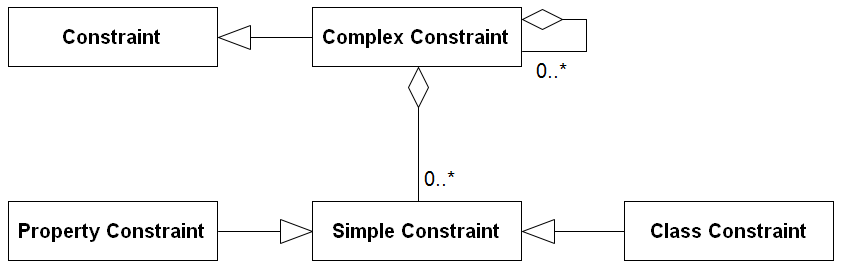
\includegraphics[width=0.80\textwidth]{images/RDF-CO-conceptual-model.png}
	\caption{RDF constraints ontology (RDF-CO) - conceptual model}
	\label{fig:RDF-CO-conceptual-model}
\end{figure}

\ms{Specific constraints} are expressed by specific constraint languages like DSP, OWL 2, ReSh, ShEx, and SPIN.
\ms{Generic constraints} are expressed by the RDF-CO.
As RDF-CO describes constraints generically, RDF-CO does not distinguish constraints according to the dimension \ms{universality}. 
The majority of constraints can be expressed in DL (see section \ref{sec:evaluation}).
In contrast, there are constraints which cannot be expressed in DL, but are also representable by the RDF-CO. 
\ms{Complex constraints} encompass \ms{simple constraints} (atomic constraints) and/or further complex constraints.
DL statements representing complex constraints are created out of DL statements representing composed constraints (if expressible in DL). 
Simple constraints may be applied to either properties (\ms{properties constraints}) or classes (\ms{class constraints}).
There are no terms representing simple and complex constraints in the RDF-CO, since context classes (associated simple constraints hold for individuals of these classes) of simple constraints may just be reused by further constraints.
As a consequence, the distinction of property and class constraints is sufficient to describe all possible RDF constraints.

\subsection{Simple Constraints (Expressible in DL)}

Sub-classes of \ms{simple constraints} are \ms{property constraints} and \ms{class constraints} (see the RDF-CO implementation model in figure \ref{fig:RDF-CO-implementation-model}). 
For both property and class constraints a context class, a list of classes, the constraining element, and the constraining value can be stated. 
Lists of left and right properties can only be stated for property constraints.

\begin{figure}
	\centering
		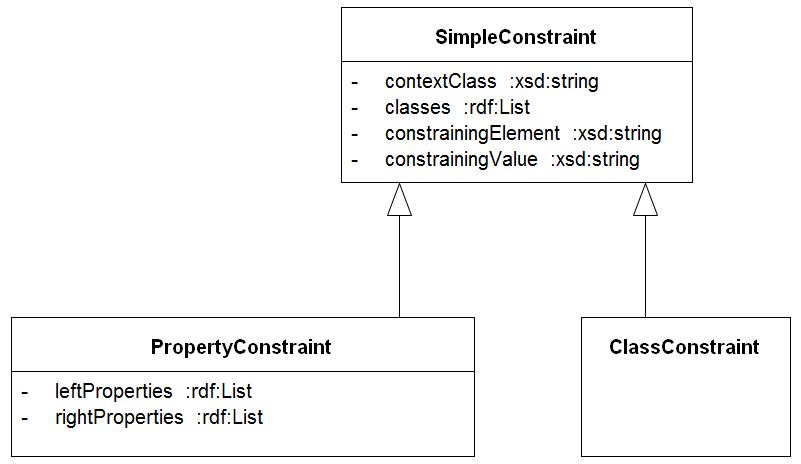
\includegraphics[width=0.70\textwidth]{images/RDF-CO-implementation-model.png}
	\caption{RDF constraints ontology (RDF-CO) - implementation model}
	\label{fig:RDF-CO-implementation-model}
\end{figure}

A constraint holds for all individuals of a context class (\ms{contextClass}).
Consider, e.g., the following cardinality restriction on the property \ms{commandsVessel}, which restricts Starfleet captains to command at least one vessel: 
\begin{DL}
$StarfleetCaptain \sqsubseteq \geq1 commandsVessel . Vessel $
\end{DL}
Mapped to the RDF-CO the cardinality restriction is classified as a property constraint which holds for individuals of the class \ms{StarfleetCaptain}:
\begin{gcotable}
property & StarfleetCaptain & commandsVessel & - & Vessel & $\geq$ & 1 \\
\end{gcotable}
The constraining element (\ms{constrainingElement}) indicates the actual type of constraint like DL concept and role constructors, (in)equality, and further keywords for constrains which cannot be expressed in DL (e.g. regular expressions and constraining facets).
In some cases, a constraint is only complete when in addition to the constraining element a constraining value (\ms{constrainingValue}) is stated.
The cardinality restriction 
\ms{$\geq$1 commandsVessel.Vessel}
constructs an anonymous class of all individuals who command at least one vessel.
Thus, the constraining element of this property constraint is the DL at-least restriction \ms{$\geq$} and the constraining value is \ms{1}.
\ms{Classes} indicate the list of classes, constraints refer to.
The qualified cardinality restriction refers to the class \ms{Vessel}, 
i.e., restricting the objects, the property \ms{commandsVessel} points to, to be of the class \ms{Vessel}.

For property constraints, left and right property lists (\ms{leftProperties}, \ms{rightProperties}) can be specified.
The assignment of properties to these lists happens relative to the constraining element - which may be an operator (e.g. $\sqsubseteq$ in case of object property paths).
\ms{Object Property Paths}\footnote{corresponds to the requirement \ms{R-55-OBJECT-PROPERTY-PATHS}} (also called complex role inclusion axioms in DL terminology)
state that, if an individual x is connected by a sequence of object properties with an individual y, 
then x is also connected with y by a particular object property. 
According to the following object property path and some instance data, lieutenant commander \ms{Data} is commanded by captain \ms{Picard} 
(as \ms{Data} is commanded by commander \ms{Riker} who is commanded by captain \ms{Picard}):
\begin{DL}
commandedByCommander $\circ$ commandedByCaptain $\sqsubseteq$ commandedByCaptain 
\end{DL}
When mapped to the RDF-CO, the properties \ms{commandedByCommander}, \ms{commandedByCaptain} are on the left side of the constraining element \ms{$\sqsubseteq$},
and the property \ms{commandedByCaptain} is on the right side:

\begin{gcotable}
property & $\top$ & commandedByCommander, commandedByCaptain & commandedByCaptain & $\top$ & $\sqsubseteq$ & - \\
\end{gcotable}

\subsection{Simple Constraints (Not Expressible in DL)}

There are simple constraints which cannot be expressed by DL such as literal pattern matching, literal value comparison, literal ranges, default values, and language tag cardinality \cite{BoschNolleAcarEckert2015}.
% maybe additional constraint default values:
% ear shape of races, e.g. vulcans / teeth color
% mathematical operations
There are multiple use cases associated with the requirement to match literals according to given patterns (\ms{Literal Pattern Matching}\footnote{corresponds to the requirement \ms{R-44-PATTERN-MATCHING-ON-RDF-LITERALS}}).
The enterprise vessel, e.g.,  can only have the registry numbers "NCC-1701", "NCC-1701-A", "NCC-1701-B", "NCC-1701-C", "NCC-1701-D", or "NCC-1701-E".
The universal restriction can be represented in DL:
\ms{Enterprise $\sqsubseteq$ $\forall$ registryNumber.RegistryNumber}.
The restriction of the datatype \ms{RegistryNumber}, however, cannot be expressed in DL, but OWL 2 DL can be used anyway to express the literal pattern matching constraint:

\begin{ex}
RegistryNumber
    a rdfs:Datatype ; owl:equivalentClass [ a rdfs:Datatype ;
        owl:onDatatype xsd:string ;
        owl:withRestrictions ( [ xsd:pattern "NCC-1701([-][A-E])?" ] ) ] .
\end{ex}

The second axiom defines \ms{RegistryNumber} as an abbreviation for a datatype restriction on \ms{xsd:string}. 
The first axiom explicitly declares \ms{RegistryNumber} to be a datatype. 
The datatype \ms{RegistryNumber} can be used just like any other datatype like in the universal restriction above.
The literal pattern matching constraint validates \ms{RegistryNumber} literals according to the stated regular expression causing a constraint violation for the triples 
\ms{Janeway commandsEnterprise Voyager} and \ms{Voyager registryNumber "NCC-74656"\textasciicircum{}\textasciicircum{}RegistryNumber}, 
but not for the triples \ms{Picard commandsEnterprise Enterprise} and \ms{Enterprise registryNumber "NCC-1701-E"\textasciicircum{}\textasciicircum{}RegistryNumber}.
The simple constraints - universal restriction and literal pattern matching - are mapped to the RDF-CO as follows:

\begin{gcotable}
property & Enterprise & registryNumber & - & RegistryNumber & $\forall$ & - \\
class & RegistryNumber & - & - & xsd:string & regex & 'NCC-1701([-][A-E])?' \\
\end{gcotable}

The \ms{Literal Pattern Matching} constraint introduces the new constraining element \ms{regex}.
For this new constraining element, the validation must be implemented.
This has to be done once for each constraint which cannot be expressed in DL.

\subsection{Complex Constraints}

\ms{Complex constraints} encompass simple constraints and/or complex constraints.
Exclusive or is a logical operation that outputs true whenever both inputs differ (one is true, the other is false).
The \ms{Context-Specific Exclusive OR of Property Groups}\footnote{corresponds to R-13-DISJOINT-GROUP-OF-PROPERTIES-CLASS-SPECIFIC} 
constraint restricts the data to contain only one of multiple property groups.
Half-Klingons, e.g., either have a klingon mother and a human father or a human mother and a klingon father, which can be expressed by ShEx:

\begin{ex}
Half-Klingon { 
    ( klingonMother Klingon , humanFather Human ) |
    ( humanMother Human , klingonFather Klingon ) }
\end{ex}

As \ms{B'Elanna Torres} is a \ms{Half-Klingon} with a klingon mother and a human father, the following data is valid:

\begin{ex}
BElannaTorres a Half-Klingon ;
    klingonMother Miral ; humanFather JohnTorres .
\end{ex}

%\begin{DL}
%rdf:type(BElannaTorres,Half-Klingon) \\
%klingonMother(BElannaTorres,Miral) \\
%klingonMother(BElannaTorres,JohnTorres)
%\end{DL}

This complex constraint can be mapped to DL:

\begin{DL}
Half-Klingon $\sqsubseteq$ ($\neg$E $\sqcap$ F) $\sqcup$ (E $\sqcap$ $\neg$F) \\ 
E $\equiv$ A $\sqcap$ B \\
F $\equiv$ C $\sqcap$ D \\
A $\sqsubseteq$ $\geq$ 1 klingonMother.Klingon $\sqcap$ $\leq$ 1 klingonMother.Klingon \\
B $\sqsubseteq$ $\geq$ 1 humanFather.Human $\sqcap$ $\leq$ 1 humanFather.Human \\
C $\sqsubseteq$ $\geq$ 1 humanMother.Human $\sqcap$ $\leq$ 1 humanMother.Human \\
D $\sqsubseteq$ $\geq$ 1 klingonFather.Klingon $\sqcap$ $\leq$ 1 klingonFather.Klingon \\
\end{DL}

The complex constraint (expressed in DL) is mapped to a generic constraint:

\begin{gcotable}
class & Half-Klingon & - & - & $\neg$E $\sqcap$ F, E $\sqcap$ $\neg$F & $\sqcup$ & - \\
class & $\neg$E $\sqcap$ F & - & - & $\neg$E, F & $\sqcap$ & - \\
class & E $\sqcap$ $\neg$F & - & - & E, $\neg$F & $\sqcap$ & - \\
class & $\neg$E & - & - & E & $\neg$ & - \\
class & E & - & - & A, B & $\sqcap$ & - \\
class & $\neg$F & - & - & F & $\neg$ & - \\
class & F & - & - & C, D & $\sqcap$ & - \\
class & A & - & - & A1, A2 & $\sqcap$ & - \\
property & A1 & klingonMother & - & Klingon & $\geq$ & 1 \\
property & A2 & klingonMother & - & Klingon & $\leq$ & 1 \\
class & B & - & - & B1, B2 & $\sqcap$ & - \\
property & B1 & humanFather & - & Human & $\geq$ & 1 \\
property & B2 & humanFather & - & Human & $\leq$ & 1 \\
class & C & - & - & C1, C2 & $\sqcap$ & - \\
property & C1 & humanMother & - & Human & $\geq$ & 1 \\
property & C2 & humanMother & - & Human & $\leq$ & 1 \\
class & D & - & - & D1, D2 & $\sqcap$ & - \\
property & D1 & klingonFather & - & Klingon & $\geq$ & 1 \\
property & D2 & klingonFather & - & Klingon & $\leq$ & 1 \\
\end{gcotable}

Even though, tools may generate generic constraints automatically, this complex constraint is composed of many other complex (e.g. minimum and maximum qualified cardinality restrictions) and simple constraints (e.g. constraints on sets).
As \ms{exact (un)qualified cardinality restrictions} and \ms{exclusive or} are frequently used complex constraints,
we propose using them as simple constraints - 	in terms of syntactic sugar.
As a consequence, the \ms{Context-Specific Exclusive OR of Property Groups} constraint above is represented as a generic constraint more intuitively and concisely:

\begin{gcotable}
class & Half-Klingon & - & - & E, F & XOR \\
class & E & - & - & A, B & $\sqcap$ \\
class & F & - & - & C, D & $\sqcap$ \\
property & A & klingonMother & - & Klingon & = & 1 \\
property & B & humanFather & - & Human & = & 1 \\
property & C & humanMother & - & Human & = & 1 \\
property & D & klingonFather & - & Klingon & = & 1 \\
\end{gcotable}

\subsection{Simple Constraints (Syntactic Sugar)}

Almost 15 percent of all RDF constraints are complex constraints which can be simplified and therefore formulated as simple constraints when using them in terms of syntactic sugar (see section \ref{sec:evaluation}).

There are three forms of RBox axioms: role inclusions, equivalences and disjointness. 
OWL provides a variety of others, namely role transitivity, symmetry, asymmetry, reflexivity and irreflexivity. 
These are sometimes considered as basic axiom types in DL as well, using some suggestive notation such as
\ms{Trans(ancestorOf)} to express that the role ancestorOf is transitive. 
However, such axioms are just syntactic sugar; 
all role characteristics can be expressed using the basic features of DL.
\ms{Irreflexive Object Properties}\footnote{corresponds to the requirement \ms{R-60-IRREFLEXIVE-OBJECT-PROPERTIES}}
restricts that an object property is irreflexive if it is never locally reflexive, i.e. no individual is connected by the object property to itself \cite{Kroetzsch2012}.
The irreflexivity constraint, stating that individuals cannot be married to themselves, can be represented in DL:

\begin{DL}
$\top$ $\sqsubseteq$ $\neg$ $\exists  marriedTo . Self$
\end{DL}

When mapped to the RDF-CO, the complex constraint aggregates three simple constraints (one property and two class constraints):

\begin{gcotable}
property & $\exists$ marriedTo . Self & marriedTo & - & Self & $\exists$ & - \\
class & $\neg$ $\exists$ marriedTo . Self & - & - & $\exists$ marriedTo . Self & $\neg$ & - \\
class & $\top$ & - & - & $\top$, $\neg$ $\exists$ marriedTo . Self & $\sqsubseteq$ & - \\
\end{gcotable}

When using the RBox axiom \ms{role irreflexivity} as syntactic sugar, 
the complex constraint transforms into a simple property constraint with exactly the same semantics:

\begin{gcotable}
property & $\top$ & marriedTo & - & - & irreflexive & - \\
\end{gcotable}

The \ms{Primary Key Properties} constraint is often useful to declare a given (datatype) property as the "primary key" of a class, so that a system can enforce uniqueness. 
Starfleet officers, e.g., are uniquely identified by their command authorization code (e.g. to activate and cancel auto-destruct sequences).
It means that the property \ms{commandAuthorizationCode} is inverse functional - mapped to DL and the RDF-CO as follows:

\begin{DL}
$(\ms{funct } commandAuthorizationCode\sp{\overline{\ }})$
\end{DL}

\begin{gcotable}
property & $\top$ & commandAuthorizationCode$^{-}$ & commandAuthorizationCode$^{-}$ & - & inverse & - \\
property & $\top$ & commandAuthorizationCode$^{-}$ & - & - & functional & - \\
\end{gcotable}

Keys, however, are even more general, i.e., a generalization of inverse functional properties \cite{Schneider2009}.
A key can be a datatype property, an object property, or a chain of properties.
For this generalization purposes, as there are different sorts of key, and as keys can lead to undecidability, 
DL is extended with \ms{key boxes} and a special \ms{keyfor} construct\cite{Lutz2005}.
This leads to the following DL and RDF-CO mappings (only one simple property constraint):

\begin{DL}
commandAuthorizationCode \ms{keyfor} StarfleetOfficer
\end{DL}

\begin{gcotable}
property & StarFleetOfficer & commandAuthorizationCode & - & - & keyfor & - \\
\end{gcotable}

%\begin{itemize}
  %\item domain and range
	%\item Primary Key Properties
	%\item ( Exact Qualified Cardinality Restrictions on Properties )
%\end{itemize}

%\subsection{Disjoint Classes}
%
%\begin{DL}
%Hologram $\sqcap$ Human $\sqsubseteq$ $\perp$\\
%Alternative:\\
%$Hologram \sqsubseteq \neg Human$
%\end{DL}
%
%\subsection{Minimum Qualified Cardinality Restrictions on Properties}
%
%\begin{DL}
%$FederationCaptain \sqsubseteq Federation \sqcap \geq1 commandsVessel . Vessel $
%\end{DL}

%\section{Transformations and Automatic Validation of Specific Constraints}
%\section{Transformations between Specific Constraints (Expressed by Different Constraint Languages)}
\section{Transformations between Specific Constraints}
\label{sec:transformations}

RDF data providers ensure that their data conforms to constraints which are part of the contract between the providers and the consumers of that data.
As there is no standard way, these constraints may be represented by multiple constraint languages (there are even more than the five promising ones\footnote{i.a. Bibframe, DQTP, Pellet ICV, RDFUnit, SPARQL, Stardog ICV}).
There is an obvious need to transform a specific constraint (\ms{$sc_{\alpha}$}) (expressed by any constraint language \ms{$\alpha$}) into a specific constraint (\ms{$sc_{\beta}$}) (expressed by any constraint language \ms{$\beta$}) - when they have the same semantics.
We use the RDF-CO as intermediate representation for these transformations.
If we define mappings ($m(sc_{\alpha}), m(sc_{\beta})$) from two equivalent specific constraints to the corresponding generic constraint (\ms{gc}),
we can convert them automatically:

\begin{DL}
$ gc = m(sc_{\alpha}) = m(sc_{\beta}) $
\end{DL}

We do not need to define mappings for each pair of semantically equivalent specific constraints.
Let's assume we are able to express a constraint by 5/6/7/8/9/10 constraint languages.
Without the intermediate generic constraint, we would have to define one mapping for each pair of specific constraints expressed by a different constraint languages
- that are \ms{\( {n \choose 2} \)} mappings for each constraint (10/15/21/28/36/45 mappings).
With an intermediate generic constraint, we only need to define \ms{n} mappings (one mapping for each specific constraint) from the specific constraints to the generic constraint (5/6/7/8/9/10 mappings).

%(n(n+1))/2

%\begin{DL}
%\(\sum \limits_{i=1}^n i = \frac{n(n+1)}{2}\)
%\(\sum \limits_{i=1}^n i\)
%\(\Binom{n}{2} \)
%\( {n \choose 2} \)
%\end{DL}

\ms{Allowed Values}\footnote{corresponds to the requirements \ms{R-30-ALLOWED-VALUES-FOR-RDF-OBJECTS} and \ms{R-37-ALLOWED-VALUES-FOR-RDF-LITERALS}}
is a common requirement to narrow down the value space of a property by an exhaustive enumeration of the valid values (both literals or resources). 
The Enterprise, e.g., is only commanded by the captains Archer, Kirk, and Picard.
This complex constraint is composed of the two simple constraints \ms{universal quantification} and \ms{allowed values} which can be represented in DL:

%\begin{DL}
%StarfleetCaptain $\equiv$ $\forall$ overruledBy . \{Commodore\} $\sqcup$ \{Admiral\}
%\end{DL}

\begin{DL}
Enterprise $\equiv$ $\forall$ commandedBy . \{Archer\} $\sqcup$ \{Kirk\} $\sqcup$ \{Picard\}
\end{DL}

First, we map these DL statements to two simple generic constraints corresponding to the RDF-CO (we define the class \ms{EnterpriseCaptains} by simply enumerating its instances):

%\begin{gcotable}
%property & StarfleetCaptain & overruledBy & - & CaptainOverruler & $\forall$ & - \\
%class & CaptainOverruler & - & - & \{Commodore\},\{Admiral\} & $\sqcup$ & - \\
%\end{gcotable}

\begin{gcotable}
property & Enterprise & commandedBy & - & EnterpriseCaptains & $\forall$ & - \\
class & EnterpriseCaptains & - & - & \{Archer\},\{Kirk\},\{Picard\} & $\sqcup$ & - \\
\end{gcotable}

The next step is to define one mapping for each specific constraint to the generic constraint.
The specific constraints (\ms{$sc_{OWL 2}$}, \ms{$sc_{ReSh}$}, and \ms{$sc_{ShEx}$}) expressed by OWL 2, ReSh, and ShEx look like this:

\begin{ex}
# OWL 2:
Enterprise rdfs:subClassOf [ a owl:Restriction .
    owl:onProperty commandedBy .
    owl:allValuesFrom [ a owl:Class ;
        owl:oneOf ( Archer Kirk Picard ) ] ] .
# ReSh:
Enterprise a rs:ResourceShape ; rs:property [
    rs:name "commandedBy" ; rs:propertyDefinition commandedBy ;
    rs:allowedValue Archer , Kirk , Picard ;
    rs:occurs rs:Exactly-one ; ] .
# ShEx:
Enterprise {
    commandedBy (Archer Kirk Picard) }
\end{ex}

%\begin{ex}
%# DSP:
%[ a dsp:DescriptionTemplate ;
    %dsp:resourceClass StarfleetCaptain ; 
    %dsp:statementTemplate [ a dsp:NonLiteralStatementTemplate ; 
        %dsp:property overruledBy ; 
        %dsp:nonLiteralConstraint [ a dsp:NonLiteralConstraint ;
            %dsp:valueClass Commodore , Admiral ] ] ] .
%# OWL 2:
%StarfleetCaptain rdfs:subClassOf [ a owl:Restriction .
    %owl:onProperty overruledBy .
    %owl:allValuesFrom [ a owl:Class ;
        %owl:oneOf ( Commodore Admiral ) ] ] .
%# ReSh:
%%StarfleetCaptain a rs:ResourceShape ;
    %%rs:property [
        %%rs:name "overruledBy" ; rs:propertyDefinition overruledBy ;
        %%rs:valueShape Commodore ; rs:occurs rs:Zero-or-many ; ] ;
    %%rs:property [
        %%rs:name "overruledBy" ; rs:propertyDefinition overruledBy ;
        %%rs:valueShape Admiral ; rs:occurs rs:Zero-or-many ; ] ;
%# ShEx:
%:StarfleetCaptain {
    %:overruledBy @:Commodore* , :overruledBy @:Admiral* }
%\end{ex}

\section{Validation of Specific and Generic Constraints}
\label{sec:validation}

We can provide the validation of all specific constraints (expressed by any constraint language) by defining a mapping to SPIN.
That's what we have done for all OWL 2 and DSP constructs (see section \ref{sec:implementation}).
%We do not have to define a mapping to SPIN for each specific constraint. 
%when we define a mapping to SPIN for each generic constraint.
But, if we define a mapping from a specific constraint to the corresponding generic constraint and if we define a mapping from the generic constraint to SPIN,
we do not have to define a mapping to SPIN for that specific constraint - 
we are able to validate the generic as well as the specific constraint.
As a consequence, we only have to define one SPIN mapping for each constraint corresponding to a requirement within the RDF validation requirements database.
19 of 74 RDF constraints can be expressed by at least four constraint languages \cite{BoschNolleAcarEckert2015}.
This means, that there must be 76 (four for each constraint) implementations to validate 76 specific constraints - instead of only 19 implementations (one for each generic constraint).

Within our SPIN validation environment, we define a SPIN construct template for each generic constraint\footnote{for details about the SPIN validation environment see \cite{BoschEckert2014-2}}.
A SPIN construct template contains a SPARQL CONSTRUCT query which generates constraint violation triples (\ms{spin:ConstraintViolation}) indicating the subject (\ms{spin:violationRoot}) and the properties (\ms{spin:violationPath}), causing constraint violations, and the reason why constraint violations have been raised (\ms{rdfs:label}).
A SPIN construct template creates constraint violation triples if all triple patterns within the SPARQL WHERE clause match.
The SPARQL CONSTRUCT query for the universal quantification (of the previous example in section \ref{sec:transformations}) is shown below:

\begin{ex}
CONSTRUCT {
    [   a spin:ConstraintViolation ; spin:violationRoot ?subject ;
        rdfs:label ?violationMessage ; spin:violationPath ?p1 . }
WHERE {	  
    [   a gclo:PropertyConstraint ;
        gclo:contextClass ?cc ;
        gclo:leftProperties ( ?p1 ) ;
        gclo:classes ( ?c1 ) ;
        gclo:constrainingElement "universal quantification" ] .
    [   a gclo:ClassConstraint ;
        gclo:contextClass ?c1 ;
        gclo:classes ( ?i1 ?i2 ?i3 ) ;
        gclo:constrainingElement "union" ] .				
    ?subject a ?cc ; ?p1 ?i .
    FILTER ( ?i != ?i1 && ?i != ?i2 && ?i != ?i3 ) . }
\end{ex}

As a consequence, the validation results do not differ for semantically equivalent constraints expressed by multiple constraint languages,
as we provide only one validation implementation for each generic constraint.

%\subsection{Not Allowed Values}

\section{Implementation}
\label{sec:implementation}

SPARQL is generally seen as the method of choice to validate RDF data according to certain constraints, although it is not ideal for their formulation. 
In contrast, OWL 2 and DSP constraints are comparatively easy to understand, but lack an implementation to validate RDF data. 
Bosch and Eckert\cite{BoschEckert2014-2} use SPIN as basis to define a
validation environment in which the validation of any constraint language\footnote{the only limitation is that constraint languages must be represented in RDF} can be implemented by representing them in SPARQL. 
The validation implementation of constraint languages is fully declarative,
consisting of a mapping from constraint languages to SPIN in form of SPARQL CONSTRUCT queries.
SPIN represents both the SPIN mappings and the SPARQL queries in RDF. 
Within the validation environment, we fully implemented the validation of all OWL 2 DL\footnote{OWL 2 SPIN mapping: \url{https://github.com/boschthomas/OWL2-SPIN-Mapping}} and DSP\footnote{DSP SPIN mapping: \url{https://github.com/dcmi/DSP-SPIN-Mapping}} constructs (for the complete DSP validation see \cite{BoschEckert2014-2}). 
The implementation can be tested at \url{http://purl.org/net/rdfval-demo}.
The SPIN engine checks for each resource if it satisfies all constraints (associated with its assigned classes) and generates a result RDF graph containing information about all constraint violations.

We provide a mapping from RDF-CO to SPIN\footnote{RDF-CO SPIN mapping: \url{https://github.com/boschthomas/RDF-CO-SPIN-Mapping}} in order to automatically validate each type of generic constraint (simple, complex, property, and class constraints).
Part of future work will be 
(1) to provide a GUI which generates generic constraints automatically according to inputs of domain experts who are not familiar with the formulation of constraints; 
(2) to offer bidirectional transformations between specific constraints (expressed by multiple constraint languages) and generic constraints;
(3) to provide translations between specific constraints (expressed by any specific constraint language) by using generic constraints as an intermediate transformation step.
%\begin{itemize}
	%\item to provide a GUI which generates generic constraints automatically according to inputs of domain experts who are not familiar with the formulation of constraints.
	%\item to offer bidirectional transformations between specific constraints (expressed by multiple constraint languages) and generic constraints. 
	%\item to provide translations between specific constraints (expressed by any specific constraint language) by using generic constraints as an intermediate transformation step.
%\end{itemize}
\section{Evaluation}
\label{sec:evaluation}

We evaluated to which extend the most promising five constraint languages fulfill each of the overall 74 requirements to formulate RDF constraints \cite{BoschNolleAcarEckert2015}.
If a constraint can be expressed in DL, we added the mapping to DL and to the generic constraint.
If a constraint cannot be expressed in DL, we only added the mapping to the generic constraint.
Therefore, we show that each constraint can be mapped to a generic constraint.
The following table shows the absolute numbers and the relative percentages for each of the three dimensions to classify constraints:

\begin{evaluation-generic-overview}
Property Constraints & 48 & 65 (64.86) \\
Class Constraints & 17 & 23 (22.96) \\
Property and Class Constraints & 9 & 12 (12.16) \\
\hline
Simple Constraints & 46 & 62 (62.16) \\
Simple Constraints (Syntactic Sugar) & 10 & 14 (13.51) \\
Complex Constraints & 18 & 24 (24.32) \\
\hline
DL Expressible & 51 & 69 (68.92) \\
DL Not Expressible & 23 & 31 (31.08) \\
\hline
Total & 74 & 100 \\
\end{evaluation-generic-overview}

Constraints can be classified as \ms{property constraints} and \ms{class constraints}.
Two thirds of the total amount of constraints are property constraints, one fifth are class constraints, and approx. 10\% are composed of both property and class constraints.
Constraints may be either atomic (\ms{simple constraints}) or created out of simple and/or complex constraints (\ms{complex constraints}).
Almost two thirds are simple constraints, a quarter are complex constraints.
Almost 15 percent are complex constraints which can be formulated as simple constraints when using them in terms of syntactic sugar.
Constraints can either be expressible in DL or not.
The majority - nearly 70\% - of the overall constraints are expressible in DL.	

\section{Related Work}

\section{Conclusion and Future Work}

\tb{ToDO: too much space before and after DL and table environments}
\tb{ToDo: there are no line breaks for ms environment}

\bibliography{../../literature/literature}{}
\bibliographystyle{plain}
\setcounter{tocdepth}{1}
%\listoftodos
\end{document}
